%@author: Marcin Mrugas

\documentclass{article} 
\usepackage{listings} 
\usepackage{polski} 
\usepackage{gensymb}
\usepackage[utf8]{inputenc} 
\usepackage[OT4]{fontenc} 
\usepackage{graphicx,color}

\usepackage{biblatex}
\usepackage{url} 
\DeclareUnicodeCharacter{00A0}{ }
\usepackage{indentfirst}
\DeclareUnicodeCharacter{00A0}{~}
\usepackage[pdftex,hyperfootnotes=false,pdfborder={0 0 0}]{hyperref} 

\bibliography{bibliography.bib}

\input{_ustawienia.tex}

%\author{}
%\date{}


\begin{document}

\input{_tytulowa}


\begin{figure}
\begin{center}
\includegraphics[width=0.5\linewidth, height=0.5\linewidth]{images/8alfa.jpg}
\end{center}
\caption{Przykładowy obraz wygenerowany przez napisany program.}
\end{figure}

\section{Opis}

\indent Moim zadniem było stworzenie programu, który zasymulowałby działanie tomografu komuterowego wraz ze pokazaniem singoramu oraz odwzorowaniem wygenerowanych danych za pomocą odwrotnej transformacji Radona. 

\section{Narzędzia}

\indent Do projektu użyłem Javy wraz z JavaFX do obsługi interfejsu. Projekt jest budowany za pocoą Maven'a. Użyłem także następujących bibliotek:

\begin{lstlisting}[frame=single]  
 <dependency>
	<groupId>dcm4che.tool</groupId>
	<artifactId>dcm4che-tool-dcm2jpg</artifactId>
	<version>2.0.29</version>
</dependency>
<dependency>
	<groupId>com.github.wendykierp</groupId>
	<artifactId>JTransforms</artifactId>
	<version>3.1</version>
</dependency>
\end{lstlisting}
Kolejno do wpółpracy z formatem plików DICOM oraz do transformacji Fourie'a.

\section{Przebieg programu}
Po wybraniu odpowiedniego zdjęcia algorytm symuluje przechodzenie promieni rentgena przez obraz poprzez zsumowanie wartości $b$ (brightness) z modelu $HSB$ koloru danego piksela. Kolejne piksele wchodzące w skład sumy są wybierane za pomogą algorytmu Bresenhama. Wartość sumy jest także normalizowana względen długości lini. Do projektu został wybrany model stożkowy układu emiter/detektor. Daną symulację opisują trzy parametry warunkujące rozmieszczenie emiterów i detektorów. Wartość $\alpha$ odpowiada za kąt pomiędzy kolejnymi emiterami rozmieszczonymi na okręgu. Parametr $\beta$ to ilość promieni wchodzących w skład pojedyńczego stożka. Zaś $l$ decyduje o rozpiętości stożka, przy czym w programie jest to kąt wewnętrzny. Kąt zewnętrzny rozwacria stożka możemy policzyć z twierdzenia o kącie wpisanym i środkowym. Wtedy kąt rozpiętości stożka przy emiterach wynosi $\frac{l}{2}$. Opisane zagadnienia pokazuje rysunek 2 \hyperlink{ramlak}{[1]}.

\begin{figure}
\begin{center}
\includegraphics[width=0.5\linewidth, height=0.5\linewidth]{images/alfabetal.jpg}
\end{center}
\caption{Parametry symulacji}
\end{figure}

Z obliczonych promieni powstaje singoram w którym w każdym wierszu znajdują się wartości z pojedyńczego stożka, a w każdej kolumnie wynik dla pojedyńczego promienia. Oczywście wyświetlany singoram jest unormaowany i zamieniony na przestrzeń barw $RGB$.

Z dotychczas zebranych danych tworzone jest odwzorowanie przy pomocy odwrotnej transformacji radona. Pojedyńczy wiersz singoramu jest zaminiany za pomoca transformacji Fourier'a na przesztrzeń częstotliwociową. Następnie wytłumiane są sygnały o nadłuższych okresach a uwydatniane te o najwyższych częstotliwościach, przez użycie filtru Ram-Lak'a. Następnie po zastosowaniu odwrotnej transformacji Fourier'a dane promienie są zaznaczane na nowym obrazie. Rysunek 3 przedstawia kolejnoc zastosowanych tranformacji.
\begin{figure}
\includegraphics[width=1\linewidth]{images/ramlak.png}
\caption{Kolejnoc zastosowanych transformacji $l$.}
\end{figure}
Ponieważ pojawił się problem normalizacji rysowanie najpierw odbywa się w osobnej tabeli w której są sumowane wartoci nakładanej linie po czym tablicza jest normalizowana i nakładana na docelowy obraz jako $B$ w przestrzeni barw $HSB$. Należało jeszcze zastosować korekcję gamma by przesunąć ku czerni szrą powiatę, oraz by uwydatnić janiesze punkty. Dodałem także opcję thresholdingu najciemniejszych punktów, gdyż  w trackie rozwiazywania problemów związanych z powiatą była to jedna z możliwości polepszenia jakści obrazu. Okazuje się jednak że treshholding na poziomie 10\% obrobinę zmniejsza błąd odwzorowania.  Interfejs użytkownika umożliwia zmianę parametrów, jednak po włączeniu programu mają one ustawione najkorzystniejsze wartości i mogłby zostać ustawione w ten sposób na stałe.
\begin{figure}
\begin{center}
	 \begin{tabular}{cc}
\includegraphics[ height=0.9\linewidth]{images/sinogram.png} &
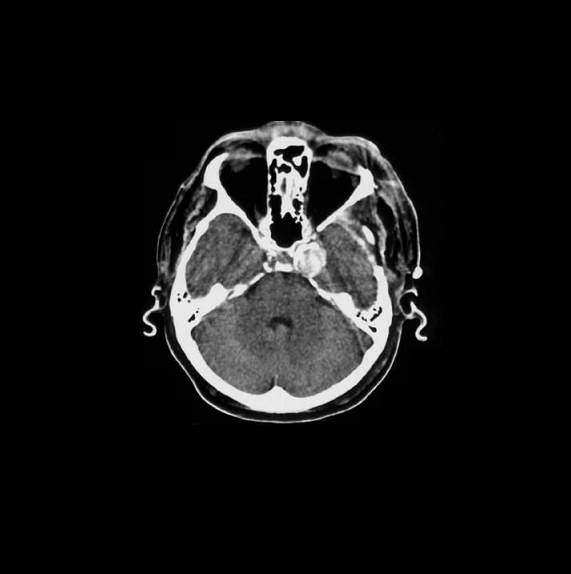
\includegraphics[width=0.5\linewidth, height=0.5\linewidth]{images/head.png}
	\end{tabular}
\end{center}
\caption{Singoram oraz wejściowy obrazu}
\end{figure}

\section{Statystyki}
\indent Ważnym aspektem było także pokazanie jak kolejne parametry wpływają na jako wygenerowanego odzworowania.

\begin{table}[h]
\caption{Jakość wygenerowanych obrazów}
	 \begin{tabular}{cccccc}
     \includegraphics[width=0.16\linewidth, height=0.16\linewidth]{images/45alfa.jpg} & 
     \includegraphics[width=0.16\linewidth, height=0.16\linewidth]{images/25alfa.jpg}  &
     \includegraphics[width=0.16\linewidth, height=0.16\linewidth]{images/8alfa.jpg} &
     \includegraphics[width=0.16\linewidth, height=0.16\linewidth]{images/3alfa.jpg}  &
     \includegraphics[width=0.16\linewidth, height=0.16\linewidth]{images/0,65alfa.jpg} &
     \includegraphics[width=0.16\linewidth, height=0.16\linewidth]{images/0,2alfa.jpg} 
     \tabularnewline
     $ \alpha = 45^{\circ} $ &
     $ \alpha = 25^{\circ} $ &
     $ \alpha = 8^{\circ} $ &
     $ \alpha = 3^{\circ} $ &
     $ \alpha = 0.65^{\circ} $ &
     $ \alpha = 0.2^{\circ} $ 
     \tabularnewline
     \includegraphics[width=0.16\linewidth, height=0.16\linewidth]{images/10beta.jpg} & 
     \includegraphics[width=0.16\linewidth, height=0.16\linewidth]{images/33beta.jpg}  &
     \includegraphics[width=0.16\linewidth, height=0.16\linewidth]{images/55beta.jpg}  &
     \includegraphics[width=0.16\linewidth, height=0.16\linewidth]{images/107beta.jpg}  &
     \includegraphics[width=0.16\linewidth, height=0.16\linewidth]{images/470beta.jpg}  &
     \includegraphics[width=0.16\linewidth, height=0.16\linewidth]{images/1000beta.jpg} 
     \tabularnewline
     $ \beta = 10 $ &
     $ \beta = 33 $ &
     $ \beta = 55 $ &
     $ \beta = 107 $ &
     $ \beta = 470 $ &
     $ \beta = 0.2 $ 
     \tabularnewline
     \includegraphics[width=0.16\linewidth, height=0.16\linewidth]{images/1l.jpg} & 
     \includegraphics[width=0.16\linewidth, height=0.16\linewidth]{images/16,5l.jpg}  &
     \includegraphics[width=0.16\linewidth, height=0.16\linewidth]{images/45l.jpg}  &
     \includegraphics[width=0.16\linewidth, height=0.16\linewidth]{images/80l.jpg}  &
     \includegraphics[width=0.16\linewidth, height=0.16\linewidth]{images/175l.jpg}  &
     \includegraphics[width=0.16\linewidth, height=0.16\linewidth]{images/250l.jpg} 
     \tabularnewline
     $ l = 1^{\circ} $ &
     $ l = 16.5^{\circ} $ &
     $ l = 45^{\circ} $ &
     $ l = 80^{\circ} $ &
     $ l = 175^{\circ} $ &
     $ l = 250^{\circ} $ 	
	\end{tabular} 
\end{table}

Kolejne odwzorowanie obrazu są pokazane w tabeli 1. W pierwszym przypadku ze zmiennym parametrem $\alpha$ wartość $\beta$ = 150, zaś $ l = 250^{\circ}$. W Drugim wierszy zminiana była wartość $\beta$ przy stałych wartościach $\alpha = 3^{\circ}$ oraz $ l = 250^{\circ}$. W ostatnim wierszy zmianana była wartość $l$ przy $\alpha = 3^{\circ}$ i $beta = 150$

Rysunek 5, 6 oraz 7 pokazują wartość błędu odwzorowania w zależności od parametrów $\alpha$, $\beta$ oraz $l$. Błąd to obliczony błąd średniokwadratowy pomiędzy wejściwoym obrazem a obrazami wyjściowymi w wersji z filtracją oraz bez.
\begin{figure}
\centering
\includegraphics[width=1\linewidth]{images/alfaPlot.png} 
\caption{Wykres błędu odwzorowania w zależnoci od parametu $\alpha$.}
\end{figure}
\begin{figure}
\includegraphics[width=1\linewidth]{images/betaPlot.png}
\caption{Wykres błędu odwzorowania w zależnoci od parametu $\beta$.}
\end{figure}
\begin{figure}
\includegraphics[width=1\linewidth]{images/lPlot.png}
\caption{Wykres błędu odwzorowania w zależnoci od parametu $l$.}
\end{figure}

\begin{thebibliography}{9}

\bibitem{FBP} \hypertarget{ramlak}{} University of Antwerp, Belgium Filtered Backprojection (FBP), 2015, \url{https://www.youtube.com/watch?v=pZ7JlXagT0w}.

\end{thebibliography}

\end{document}

